\documentclass{beamer}
% From share latex templates  - default presentation 
% Choose how your presentation looks.
%
% For more themes, color themes and font themes, see:
% http://deic.uab.es/~iblanes/beamer_gallery/index_by_theme.html
%
\mode<presentation>
{
  \usetheme{Boadilla}      % or try Darmstadt, Madrid, Warsaw, ...
  \usecolortheme{owl} % or try albatross, beaver, crane, ...
  \usefonttheme{serif}  % or try serif, structurebold, ...
   \setbeamertemplate{navigation symbols}{}
  \setbeamertemplate{caption}[numbered]
} 

\usepackage{tikz}
\usepackage{tikz}
\usepackage{graphicx}
\newcommand*{\ClipSep}{0.09cm}%
\newcommand{\rlogo}[3]{%
\begin{tikzpicture}
\node [inner sep=#1] at (0,0) {\includegraphics[width=#2]{#3}};
\draw [white, rounded corners=\ClipSep, line width=\ClipSep] 
    (current bounding box.north west) -- 
    (current bounding box.north east) --
    (current bounding box.south east) --
    (current bounding box.south west) -- cycle
    ;
\end{tikzpicture}}

\newcommand{\mylogo}[3]{%
	\tikz\node[draw,thick,inner sep=2pt,rounded corners=#1,text=white,path picture={\node at (path picture bounding box.center){\includegraphics[width=#2]{#3}};}]{};
}%
\usepackage[percent]{overpic}
\usepackage[english]{babel}
\usepackage[utf8x]{inputenc}
\usepackage{fontspec}
\setmainfont{Michroma}
%\setmainfont{Courier}
\usebackgroundtemplate%
{%
    
\includegraphics[width=\paperwidth,height=\paperheight]{./back_net.jpg}%
}

\makeatletter
\gdef\@ptsize{2} % 1 for 11pt doc, 2 for 12pt
\makeatother
\usepackage{setspace}
\doublespace

\newcounter{saveenumi}
\newcommand{\seti}{\setcounter{saveenumi}{\value{enumi}}}
\newcommand{\conti}{\setcounter{enumi}{\value{saveenumi}}}
\resetcounteronoverlays{saveenumi}

\title[Linux: Get Your Feet Wet]{Linux : Get your feet wet}
\author{Bridge Course '19}
\institute{EE Dept IITB}
\date{24 July 2019}

\begin{document}

\begin{frame}
\begin{center}

\includegraphics[scale=0.5]{./gnome_logo.png}%
\end{center}
\titlepage
\end{frame}

% Uncomment these lines for an automatically generated outline.
\begin{frame}{Outline}
  \tableofcontents
\end{frame}

\section{Introduction}
\subsection{What is Linux}


\begin{frame}
\textbf{Linux is a family of open source Unix-like operating systems based on the Linux kernel, Typically packaged in a Linux distribution}
\vskip 1cm
\rlogo{1pt}{2.0cm}{./ubuntu.png}
\rlogo{1pt}{2.0cm}{./centos.png}
\rlogo{1pt}{2.0cm}{./fedora.jpeg}
\rlogo{1pt}{2.0cm}{./arch.jpeg}
\rlogo{1pt}{2.0cm}{./lubuntu.png}
\newline
\rlogo{1pt}{2.0cm}{./rhel.png}
\rlogo{1pt}{2.0cm}{./kali3.jpeg}
\rlogo{1pt}{2.0cm}{./debian.png}
\rlogo{1pt}{2.0cm}{./mate.png}
\rlogo{1pt}{2.0cm}{./suse.png}
%\begin{block}{Examples}
%Some examples of commonly used commands and features are included, to help you get started.
%\end{block}

\end{frame}
\subsection{Why Linux}
\begin{frame}{Why Linux}
\begin{enumerate}
	\item<2-> Access to hardware - almost no restrictions
	\item<3-> Opensource - view code , modify , learn create
	\item<4-> Tailor Made - servers , fedora scientific
	\item<5-> Top 100 fastest supercomputers run linux 
	\item<6-> Almost all tech giants funds linux development
\end{enumerate}
\end{frame}
\begin{frame}{Why Linux ctd..}
\begin{enumerate}
	\item<2-> Free
	\item<3-> Sabko Cadence chalana he
	\item<4-> Friends urge friends to use linux 
	\item<5-> Microsoft gives you windows. Linux gives you whole house
\end{enumerate} 
\end{frame}
\section{Linux Basics}
\subsection{Linux File System}
{
	%\usebackgroundtemplate%
	%{%
	 %   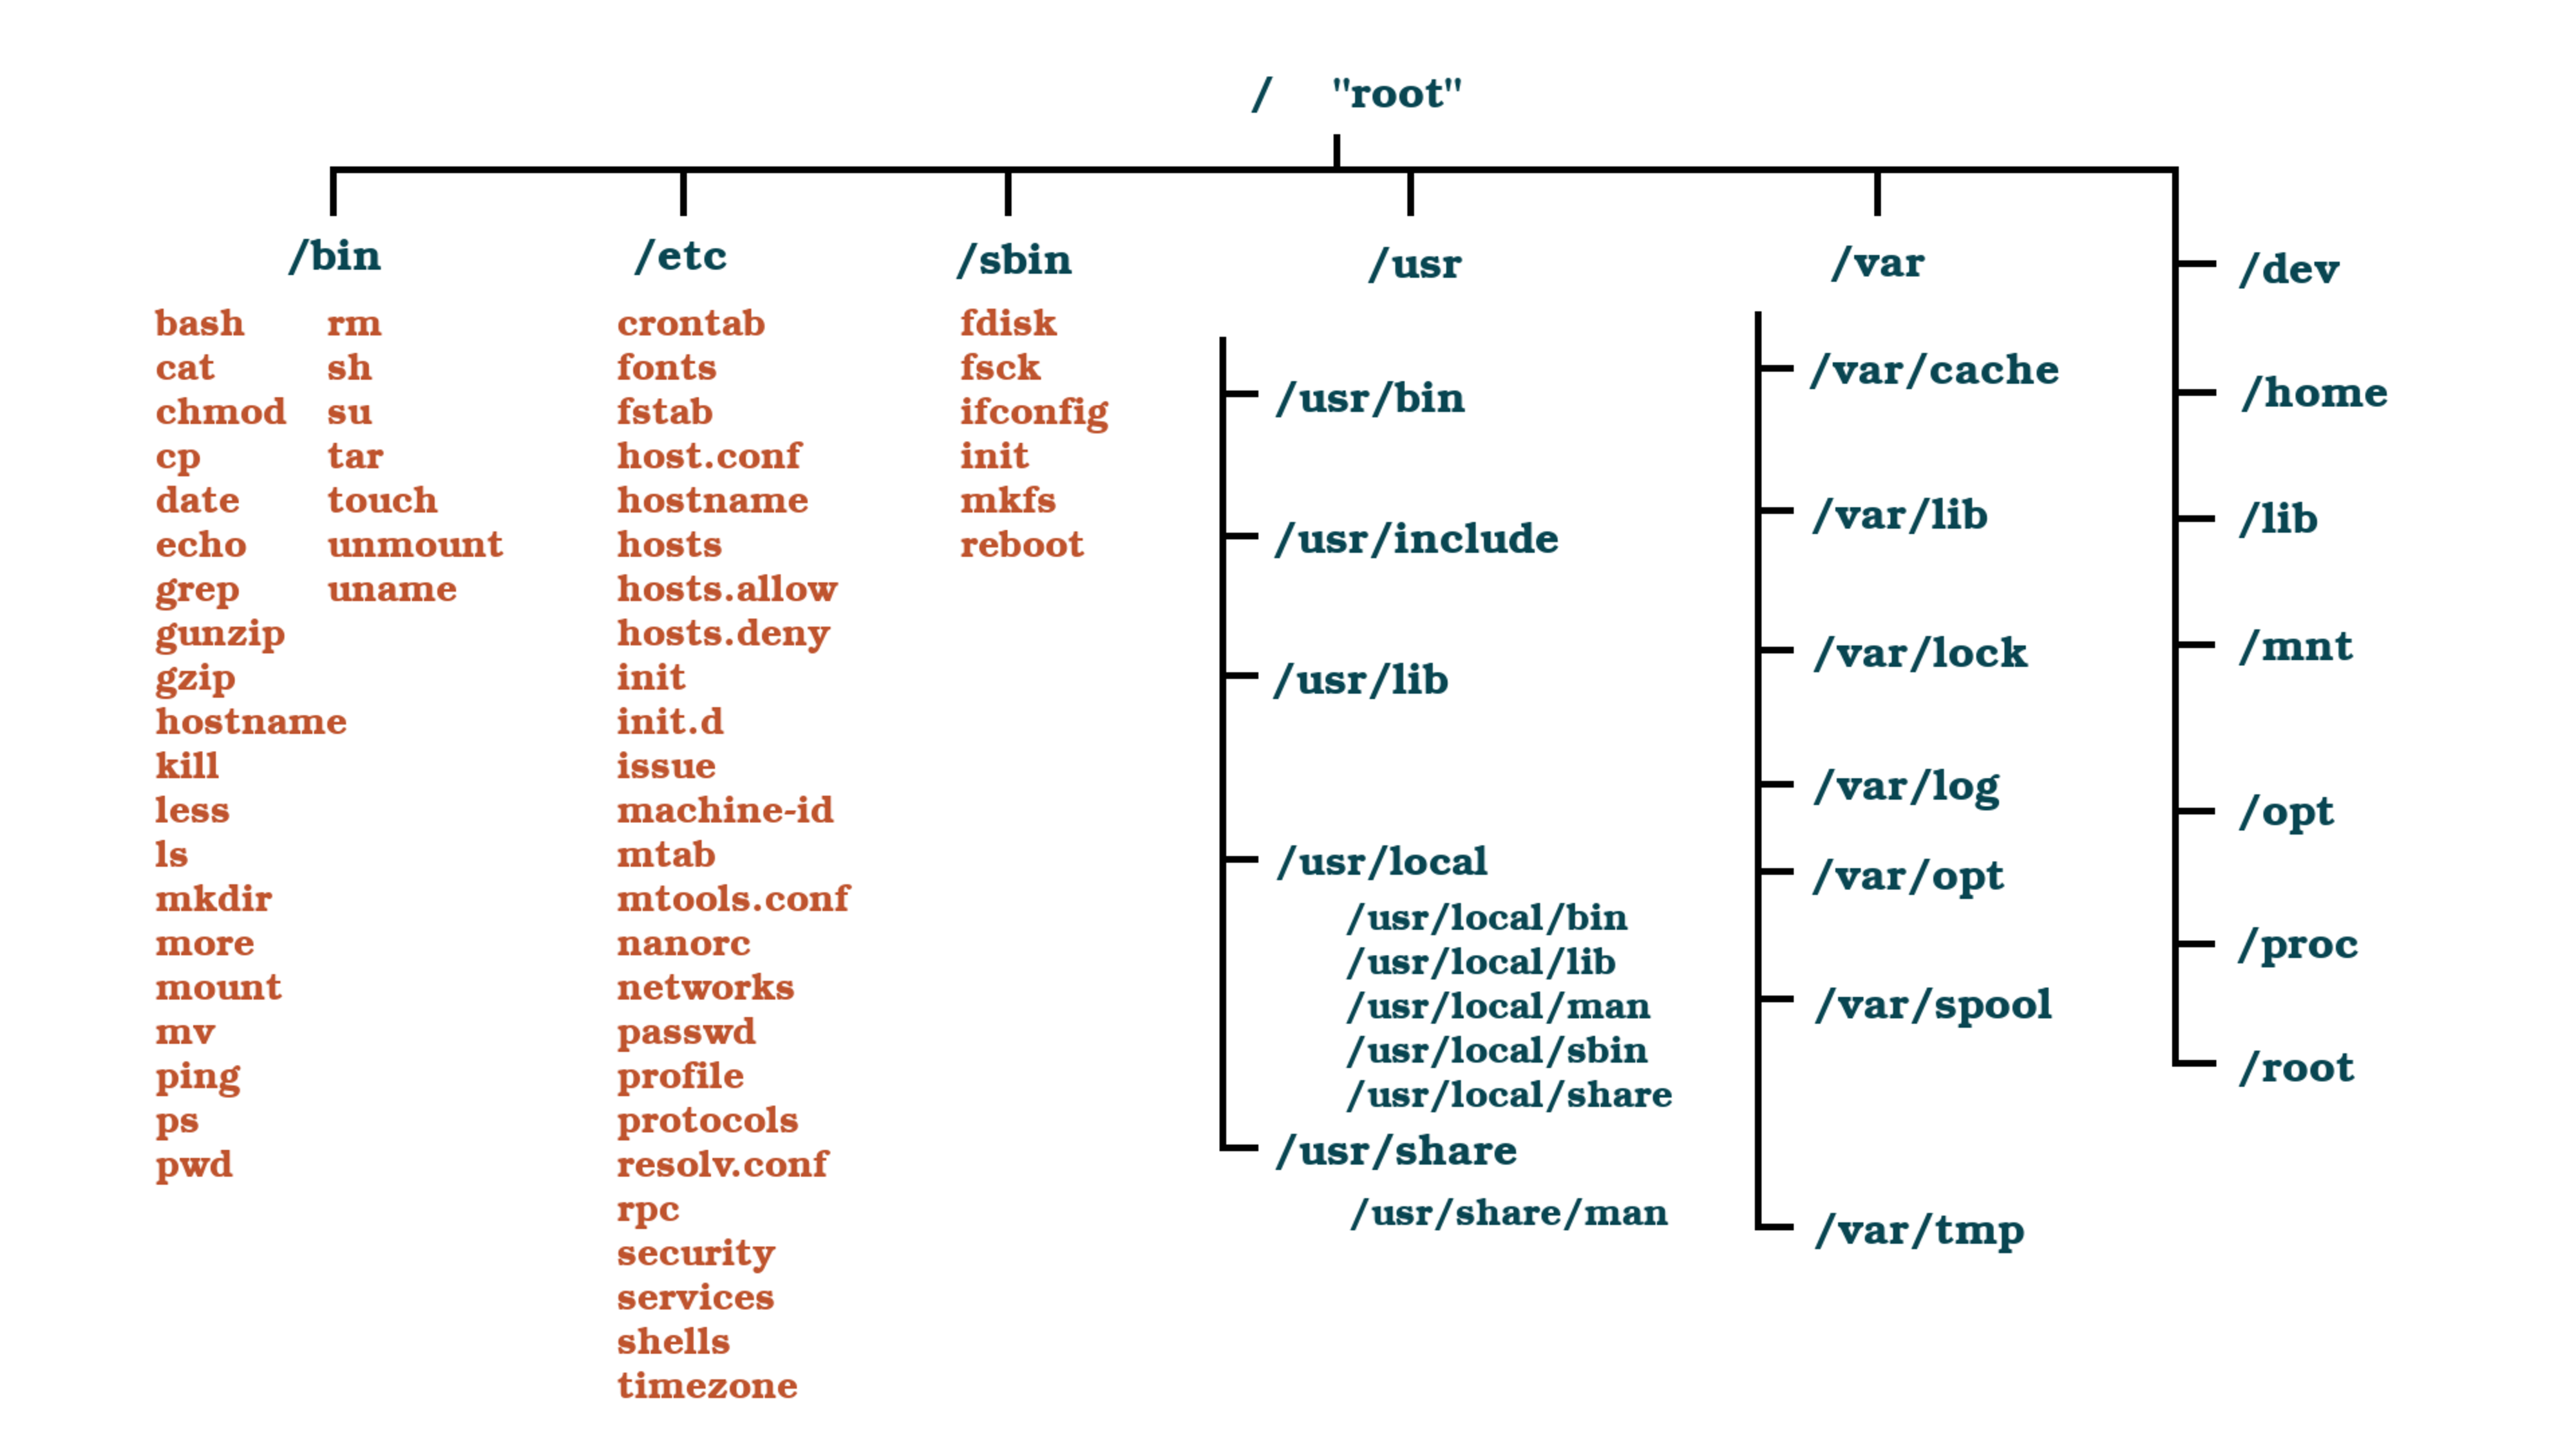
\includegraphics[height=0.8\textheight]{./filesystem.pdf}%
	%}

	\begin{frame}{File System Hierarchy}
		\begin{figure}
			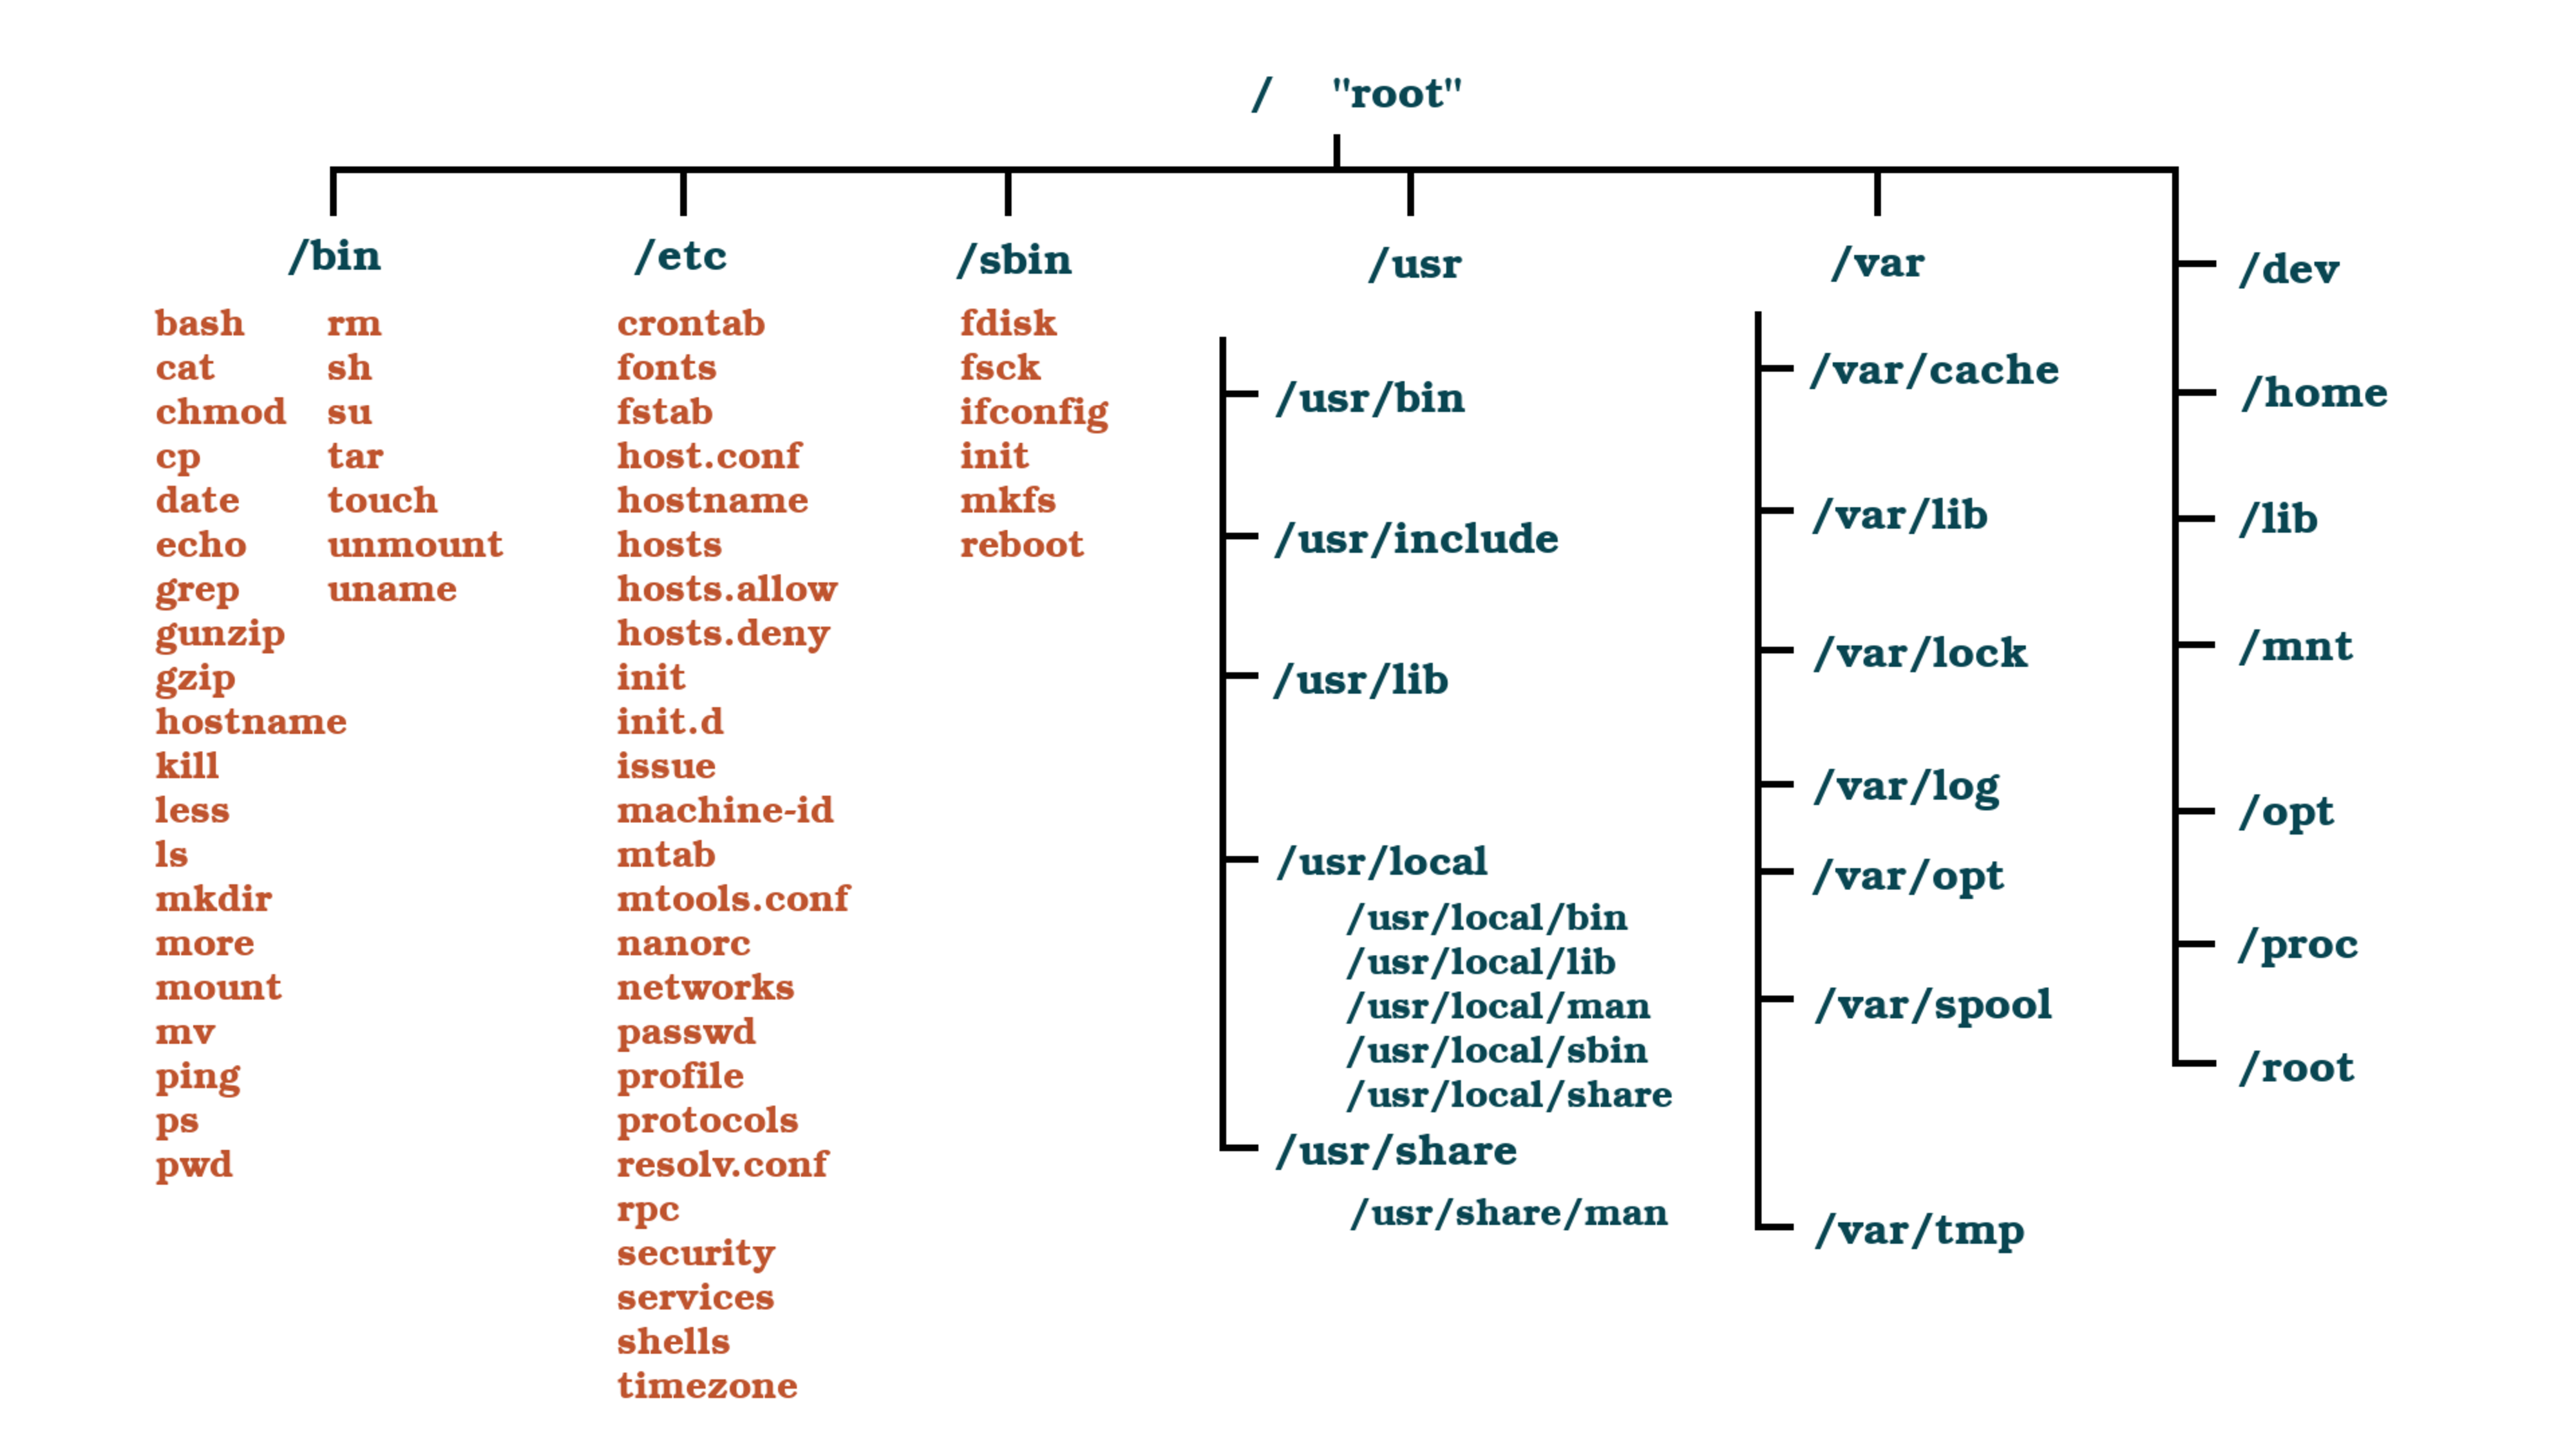
\includegraphics[width=0.9\paperwidth,height=0.8\paperheight]{./filesystem.pdf}
		\end{figure}
	\end{frame}
}

{\fontfamily{Serif}\selectfont
\begin{frame}{Linux File System:  Basic commands}
\begin{enumerate}
	\item<2->ls  - list the files the current directory
	\item<3->pwd - print the working directory
	\item<4->touch <file\_name> - create an empty file 
	\item<5->mkdir <dir\_name> - create a directory
	\item<6->cd 	- change directory 
\end{enumerate}
	\begin{alertblock}{Note}
		{use : man <command> - to get the full details regarding any command }
	\end{alertblock}
\end{frame}
}
{
	\usebackgroundtemplate%
	{%
	    
\includegraphics[width=\paperwidth,height=\paperheight]{./back_net.jpg}%
	}
\fontfamily{Serif}\selectfont
\begin{frame}{Users, Group and Permissions}
	As we saw, everything can be treated as a file in linux. \\
	\pause
	Who has permissions to edit these files???\\
	\pause
	For each file, linux assigns a set of attributes , some of these decides which users can {\textbf{Read , Write}} and (if possible )\textbf{Execute} the file. These attributes are called the file permissions. \\
	\pause
	For each file, permissions are given in three categories.
			
\end{frame}
\begin{frame}{Users, Group and Permissions}
\begin{center}
		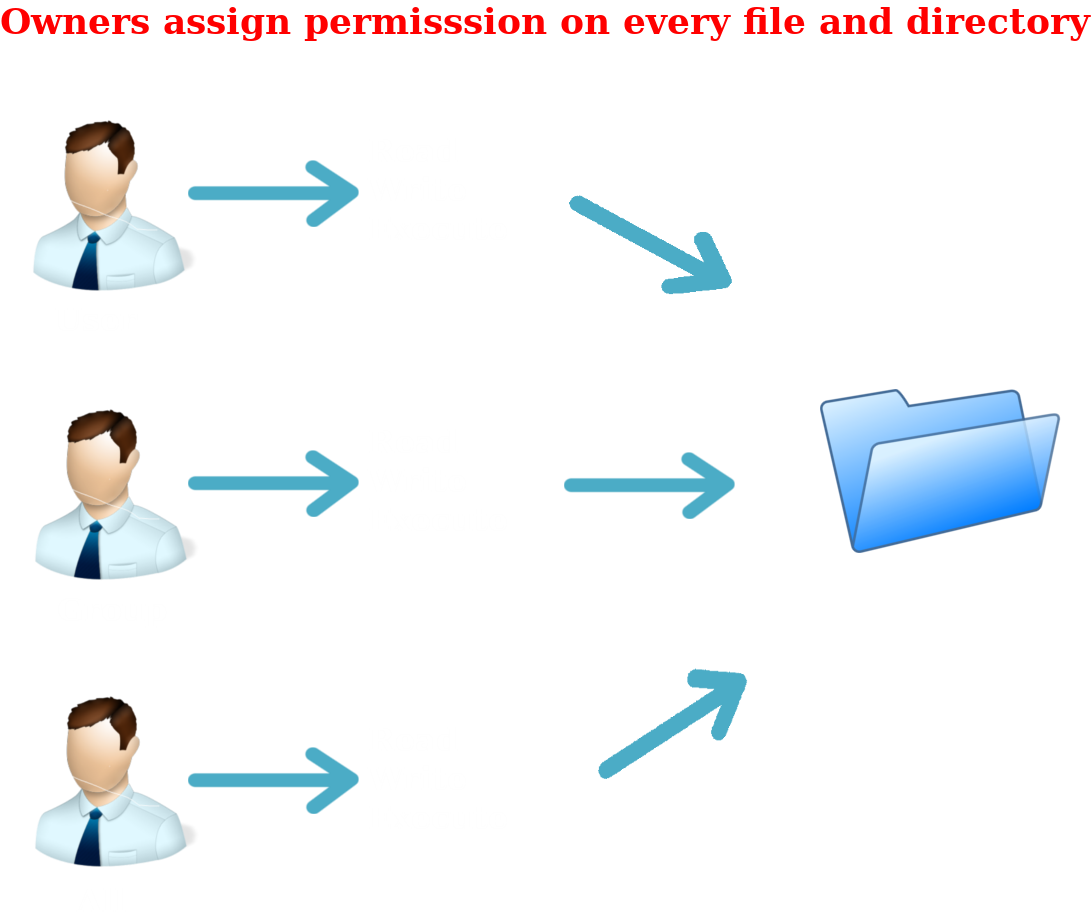
\includegraphics[scale=0.16]{./file_permissions2.png}%
\end{center}
\end{frame}

%	\vskip 1cm
	\begin{frame}{TODO}
		\begin{block}{hint}
		OWNER|GROUP|ALL. \\
		RWX-RWX-RWX\\
		\end{block}
		\begin{enumerate}
			\item<1->	use ls -l command to find out permission of files given to you.
			\item<2->	try executing 
			\item<2->		./hello\_perm.sh 
			\item<2->	what do you see	
			\seti		
		\end{enumerate}

	\end{frame}
	
	\begin{frame}
		\begin{enumerate}
			\conti
			\item<1->	change permission the file using 
			\item<1->		chmod 111 hello\_perm.sh
			\item<1->	try executing now  . 
			\item<2->	try to read file using 
			\item<2->	cat hello\_perm.sh
			\item<2->		chmod 755 hello\_perm.sh 
			\item<2->	cat hello\_perm.sh
		\end{enumerate}
	\end{frame}
}
\section{Standard out and IO redirection}
{
	\fontfamily{Serif}\selectfont
\begin{frame}{Echo and output redirection}
	\begin{enumerate}
		\item<1-> echo "test"
		\item<2-> output redirection (w+), echo "to file" > test-file
		\item<3-> appeding (a+), echo "added new line " >> test-file
		\item<4-> substitutions, echo `pwd`
			\item<5-> substitutions , echo `cat test-file`
		\item<5-> echo "current directory is `pwd`"
	\end{enumerate}
\end{frame}
\begin{frame}{cut command}
	Cut command is used to extract one or more fields from a file with fields seperated by a delimiter\\
	use cat  to view the contents of examples/cut-input\\ \pause
	cut syntax - cut -d '<delimiter>' -f<number> <filename>\\
	try printing out only the names\\ \pause
	ans : cut -d ',' -f1 cut-input\\
	what is the command to get only specialisation ? \pause


\end{frame}
\begin{frame}{sort command}
	sort can be applied on any of the fields\\ \pause 
	sort syntax - sort -t '<delimiter>' -k<number> <filename>\\
	try sorting based the names\\ \pause
	ans : sort -t ',' -k1\\
	what is the command to get only specialisation ? \pause


\end{frame}
\begin{frame}{grep command}
	grep is used for finding occurences\\ 
	\begin{enumerate}
		\item<2-> grep <find> <filename>
		\item<2-> grep pclab cut-input1
		\item<3-> grep -i variant 
		\item<4-> grep -i ee5 cut-input2 -c 
		\item<5-> grep with regexes 
	\end{enumerate}


\end{frame}
\begin{frame}{pipes(|) and the Unix philosophy}
	Pipe allows us to redirect the output of one command as the input of another command\\ 
	common syntax -   command1 input-file | command2 \\
	eg: cat test-file | sort \\
	Q: write the command to get only the sorted names from file cut-input2\\
	use cat cut-input2 to inspect the file\\ \pause
	ans : cut -d ',' -f1 cut-input2 | sort \\
	what is the command to sort all lines based on names for EE1?\\ \pause
	grep -i ee1 | sort -t ',' -k1 


\end{frame}
}

\section{Git Basics}
{
\subsection{Git - What \& Why?}

\begin{frame}{Git - What \& Why?}
	\begin{enumerate}
		\item<2-> Version control system
		\item<2-> Manages source code history
		\item<2-> Git is local
		\item<3-> Free and open source
		\item<3-> Fast and small		
	\end{enumerate}
\end{frame}

\begin{frame}{GitHub}
	\begin{enumerate}
		\item<2-> Git-based repository hosting platform with over 26 million users
		\item<3-> GitHub projects can be made public and every publicly shared code is freely open to everyone
		\item<4-> You can have private projects as well
		\item<5-> Can be used for issue tracking, documentation, and wikis
	\end{enumerate}
\end{frame}

\begin{frame}{Other Git repo hosting platforms}
	\begin{enumerate}
		\item AWS codecommit
		\item Gitlab - you can also create your own git server using gitlab
		\item Bitbucket
		\item Sourceforge
		\item ...
		\item git.ee.iitb.ac.in 
	\end{enumerate}
\end{frame}

\subsection{Git - Getting Started}

\begin{frame}{Getting Started}
	\begin{enumerate}
		\item<2-> Install git
		\item<2-> sudo apt install git-all
		\item<3-> Check installation
		\item<3-> git -- --version		
	\end{enumerate}
\end{frame}

\begin{frame}{Getting Started}
	\begin{enumerate}
		\item<2-> Cloning a repository
		\item<2-> git clone repo-address
		\item<2-> Eg. git clone https://github.com/aswinpajayan/linux-workshop.git
		\item<3-> Adding the changes
		\item<3-> git add updated-filename
		\seti
	\end{enumerate}
\end{frame}

\begin{frame}{Getting Started}
	\begin{enumerate}
		\conti
		\item<2-> Committing changes
		\item<2-> git commit -m "Commit message"
		\item<3-> Pushing changes to remote repository
		\item<3-> git push origin branch-name
		\item<4-> Pulling latest changes from remote repository
		\item<4-> git pul origin branch-name
		\seti
	\end{enumerate}
\end{frame}

\begin{frame}{Getting Started}
	\begin{enumerate}
		\conti
		\item<2-> Other useful commands
		\item<2-> git branch
		\item<2-> git status
		\item<2-> git diff filename
	\end{enumerate}
\end{frame}

}

\section{Running python code}
{
	\subsection{Running python code}
	\begin{frame}{Running python code}
		\begin{enumerate}
		\item<2-> Install Python
		\item<3-> For Python 3: python3 <filename>.py
		\item<3-> For Python 2: python <filename>.py
			\end{enumerate}
	\end{frame}		
}

\section{Facilities Provided by EE Dept}
{
\begin{frame}{Facilities Provided by EE Dept}
	\begin{enumerate}
		\item<2-> Matlab Servers - Ravan and Rudra
		\item<2-> Ravan - 10.107.1.5
		\item<2-> Rudra - 10.107.1.6
		\item<3-> Personal web page hosting								\item<4-> EE Student email
		\item<5-> PC Lab, 1st Floor, EE Dept.
		\seti
	\end{enumerate}
\end{frame}

\begin{frame}{Facilities Provided by EE Dept}
	\begin{enumerate}
		\conti
		\item<2-> For more details : Visit PCLab FAQ
		\item<2-> \url{https://www.ee.iitb.ac.in/pclab_faq/}
		\item<3-> Use : Thunderbird
	\end{enumerate}
\end{frame}
}
\end{document}

